%!TEX root = ../BUSystematics.tex

\graphicspath{{Body/Figures/CBO/}{Body/Figures/CBO/Frequency/}{Body/Figures/CBO/TimeConstants/}}

\clearpage
\section{CBO Systematic Errors}

\subsection{Frequency Change}


The systematic error due to the fixed CBO frequency model is calculated as the \DR with the Tracker Station 12 vs Tracker Station 18 parameters. These parameters are given in \refref{CBOFreqTrackingElog}, and the Endgame parameters are shown in \figref{fig:CBOFreq}. \tabref{tab:systematicError_CBOFreq} gives the systematic errors.

The HighKick and 9d Ratio results are less affected, presumably because the lifetime is fixed in those fits and there is a correlation.


\begin{figure}[h]
    \centering
    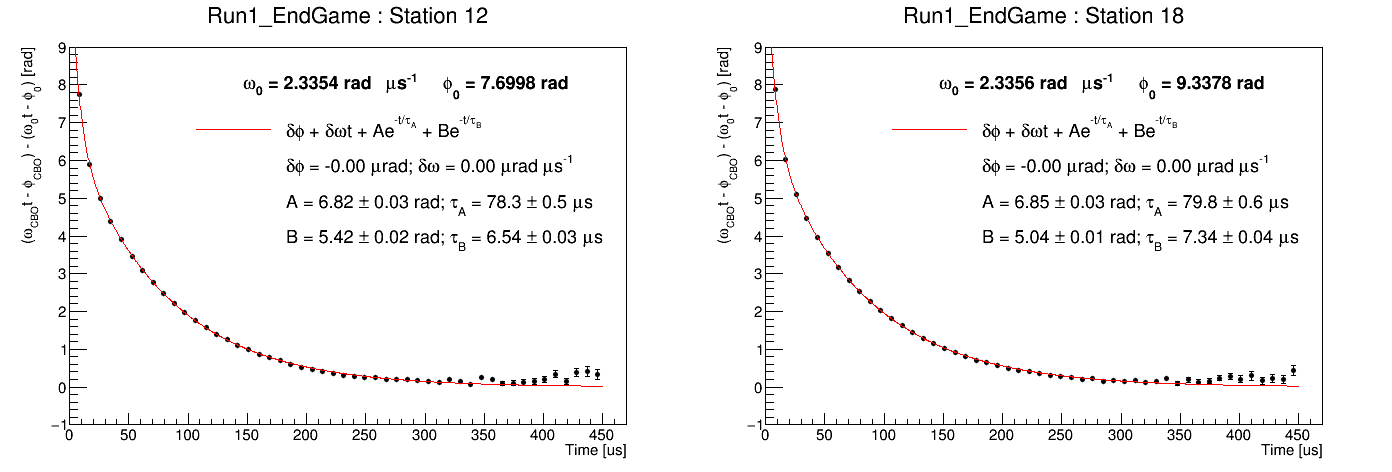
\includegraphics[width=\textwidth]{Run1_EndGame_CBOFreq}
    \caption[]{CBO frequency parameters for the Endgame dataset as determined in the tracking analysis. The y axis is in units of ... (see thesis description)}
    \label{fig:CBOFreq}
\end{figure}


\begin{table}[h]
\centering
\renewcommand{\arraystretch}{1.2}
\begin{tabularx}{0.65\linewidth}{@{\extracolsep{\fill}}XYY}
  \hline
    \multicolumn{3}{c}{\textbf{Systematic Error due to CBO Frequency}} \\
  \hline\hline
    Dataset & \thead{T-Method} & \thead{R-Method} \\
  \hline
    60h & 10.9 & 5.3 \\
    HighKick & 22.5 & 0.7 \\
    9d & 21.3 & 1.6 \\ 
    Endgame & 22.2 & 8.5 \\
  \hline
\end{tabularx}
\caption[Systematic error due to CBO frequency]{Systematic error due to CBO frequency. Units are in ppb.}
\label{tab:systematicError_CBOFreq}
\end{table}




\clearpage
\subsection{Decoherence Envelope}


The systematic error from the CBO decoherence envelope was estimated by introducing a constant $C$ in the CBO function part of the fit equation and then looking at the \DR. This constant was allowed to float...


might want to include figure of amplitude shape like in thesis showing the C constant is a reasonable adjustment

\begin{table}[h]
\centering
\setlength\tabcolsep{10pt}
\renewcommand{\arraystretch}{1.2}
\begin{tabularx}{0.6\linewidth}{XYYY}
  \hline
    \multicolumn{4}{c}{\textbf{Fitted CBO envelope constants}} \\
  \hline\hline
    Dataset & \thead{Fit Method} & \multicolumn{1}{c}{$C$} & \multicolumn{1}{c}{$\delta C$} \\
  \hline
    \multirow{2}{*}{60h} & \thead{T} & 7.1 & 4.0 \\
                         & \thead{R} & 16.1 & 5.1 \\
  \hline
    \multirow{2}{*}{HighKick} & \thead{T} & 5.2 & 1.8 \\
                              & \thead{R} & 15.7 & 11.2 \\
  \hline
    \multirow{2}{*}{9d} & \thead{T} & 7.8 & 2.9 \\
                        & \thead{R} & 13.7 & 12.3 \\
  \hline
    \multirow{2}{*}{Endgame} & \thead{T} & 5.5 & 2.1 \\
                             & \thead{R} & 10.9 & 3.4 \\
  \hline
\end{tabularx}
\caption[]{Units are in 1e-4.}
\label{tab:CBOenvConstants}
\end{table}





\begin{table}
\centering
\renewcommand{\arraystretch}{1.2}
\begin{tabularx}{\linewidth}{@{\extracolsep{\fill}}XYY}
  \hline
    \multicolumn{3}{c}{\textbf{Systematic Error due to CBO Decoherence Envelope}} \\
  \hline\hline
    Dataset & \thead{T-Method} & \thead{R-Method} \\
  \hline
    60h & 38.3 & 5.5 \\
    HighKick & 3.7 & 9.1 \\
    9d & 13.4 & 0.2 \\ 
    Endgame & 3.3 & 5.9 \\
  \hline
\end{tabularx}
\caption[Systematic error due to CBO decoherence envelope]{Systematic error due to CBO decoherence envelope. Units are in ppb.}
\label{tab:systematicError_CBOenvelope}
\end{table}



\clearpage
\subsection{Time Constants}

In the fit function the N, asymmetry, and phase terms all have CBO modifications to them, where there are new cbo amplitude and phase paramters for each parameter. The lifetime is typically fixed to be the same in all cases. However it has been claimed that the CBO lifetime on the asymmetry and phase CBO terms could be as much as 50\% different from that of the N term. In order to evaluate a systematic error due to this possibility, fits were redone by applying multipliers of 0.5 and 1.5 in the various combinations to the respective lifetimes, for a total of 4 new fits for each dataset. The maximum \DR seen from any of the combinations was then taken as the systematic error on \R. Typically the combinations of 0.5 and 1.5 produced the largest changes, as opposed to both being 0.5 or 1.5.



\begin{table}
\centering
\setlength\tabcolsep{10pt}
\renewcommand{\arraystretch}{1.2}
\begin{tabularx}{\linewidth}{@{\extracolsep{\fill}}lGGGG}
  \hline
    \multicolumn{5}{c}{\textbf{T-Method \DR with multipliers on CBO asymmetry and phase lifetimes}} \\
  \hline\hline
    Dataset & \thead{(0.5, 0.5)} & \thead{(1.5, 0.5)} & \thead{(0.5, 1.5)} & \thead{(1.5, 1.5)} \\
  \hline
    60h & -6.3 & 8.6 & \multicolumn{1}{K}{-10.8} & 4.3 \\
    HighKick & -9.6 & \multicolumn{1}{K}{23.1} & -22.7 & 9.8 \\
    9d & 15.7 & -13.0 & \multicolumn{1}{K}{23.4} & -5.7 \\ 
    Endgame & -8.2 & 5.4 & \multicolumn{1}{K}{-10.5} & 3.2 \\
  \hline
\end{tabularx}
\caption[]{\DR's for the various multiplier combinations for the T-Method fits. Multipliers are on the asymmetry and phase CBO lifetime respectively. The absolute value of the bold elements are taken as the systematic errors for the various datasets. Units are in ppb.}
\label{tab:systematicError_}
\end{table}


\begin{table}
\centering
\setlength\tabcolsep{10pt}
\renewcommand{\arraystretch}{1.2}
\begin{tabularx}{\linewidth}{@{\extracolsep{\fill}}lGGGG}
  \hline
    \multicolumn{5}{c}{\textbf{R-Method \DR with multipliers on CBO asymmetry and phase lifetimes}} \\
  \hline\hline
    Dataset & \thead{(0.5, 0.5)} & \thead{(1.5, 0.5)} & \thead{(0.5, 1.5)} & \thead{(1.5, 1.5)} \\
  \hline
    60h & -0.1 & 9.3 & \multicolumn{1}{K}{-10.8} & -1.8 \\
    HighKick & -13.1 & 18.0 & \multicolumn{1}{K}{-21.8} & 9.3 \\
    9d & -2.4 & -28.7 & \multicolumn{1}{K}{30.9} & 3.3 \\ 
    Endgame & -6.9 & 5.0 & \multicolumn{1}{K}{-9.8} & 2.3 \\
  \hline
\end{tabularx}
\caption[]{\DR's for the various multiplier combinations for the R-Method fits. Multipliers are on the asymmetry and phase CBO lifetime respectively. The absolute value of the bold elements are taken as the systematic errors for the various datasets. Units are in ppb.}
\label{tab:systematicError_}
\end{table}





\clearpage
\subsection{Time Constants Fixed}

In the HighKick and 9d datasets the CBO lifetimes in the R-Method fits are fixed to those from corresponding T-Method fits, since otherwise the fits do not like to converge to a nice value. In order to determine a systematic error from this fixed parameter, the sensitivity of \R to this fixed parameter was determined, and then multiplied against the T-Method fit error on the parameter. The scans are shown in \figref{fig:CBOfixedLifetime}. The scan results and systematic error are shown in \tabref{tab:systematicError_FixedCBOLifetime}.



\begin{figure}[h]
\centering
    \begin{subfigure}[t]{0.45\textwidth}
        \centering
        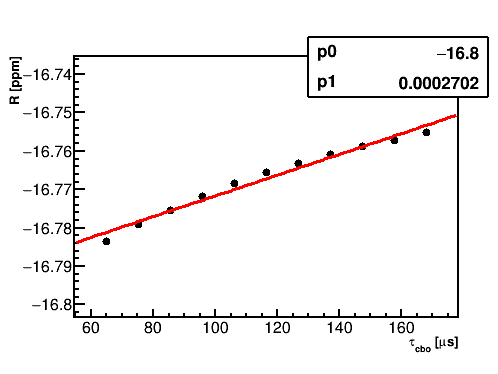
\includegraphics[width=\textwidth]{FullRatio_R_Vs_tau_cbo_Canv_HK}
        \caption{HighKick dataset.}
    \end{subfigure}% %you need this % here to add spacing between subfigures
    \hspace{1cm}
    \begin{subfigure}[t]{0.45\textwidth}
        \centering
        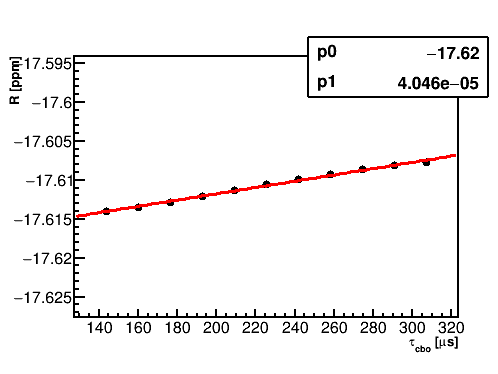
\includegraphics[width=\textwidth]{FullRatio_R_Vs_tau_cbo_Canv_9d}
        \caption{9d dataset.}
    \end{subfigure}
\caption[]{\R vs fixed CBO lifetime. The parameter $p_{1}$ is in units of ppm/microseconds.}
\label{fig:CBOfixedLifetime}
\end{figure}


\begin{table}
\centering
\renewcommand{\arraystretch}{1.2}
\begin{tabularx}{0.65\linewidth}{@{\extracolsep{\fill}}XccY}
  \hline
    \multicolumn{4}{c}{\textbf{Systematic Error due to fixed CBO lifetime}} \\
  \hline\hline
    Dataset & \thead{$dR/d\tau_{cbo}$} & \thead{T-Method $\sigma_{\tau_{cbo}}$} & \thead{R-Method \dR} \\
  \hline
    HighKick & 0.27 & 10.3 & 2.8 \\
    9d & 0.04 & 16.3 & 0.7 \\ 
  \hline
\end{tabularx}
\caption[Systematic error due to fixed CBO lifetime]{Systematic error due to fixed CBO lifetime. Units are in ppb for the error. Units are ppb per microsecond and microsecond for the other two quantities.}
\label{tab:systematicError_FixedCBOLifetime}
\end{table}
